%
% Author: David Oniani
%
%  _____    ___     _  __
% |_   _| _|_ _|___| |/ /___
%   | || '__| |/ __| ' // __|
%   | || |  | | (__| . \\__ \
%   |_||_| |___\___|_|\_\___/
%

%%%%%%%%%%%%%%%%%%%%%%%%%%%%%%%%%%%%%%%%%%%%%%%%%%%%%%%%%%%%%%%%%%%%%%%%%%%%%%%
% Document Definition
%%%%%%%%%%%%%%%%%%%%%%%%%%%%%%%%%%%%%%%%%%%%%%%%%%%%%%%%%%%%%%%%%%%%%%%%%%%%%%%

\documentclass[12pt]{article}

%%%%%%%%%%%%%%%%%%%%%%%%%%%%%%%%%%%%%%%%%%%%%%%%%%%%%%%%%%%%%%%%%%%%%%%%%%%%%%%
% Packages and Related Settings
%%%%%%%%%%%%%%%%%%%%%%%%%%%%%%%%%%%%%%%%%%%%%%%%%%%%%%%%%%%%%%%%%%%%%%%%%%%%%%%

% Global, document-wide settings
\usepackage[margin=1in]{geometry}
\usepackage[utf8]{inputenc}
\usepackage[english]{babel}

% Other essential packages
\usepackage{booktabs}
\usepackage{hyperref}
\usepackage{minted}
\usepackage{tocloft}
\usepackage{xcolor}

% Packages for making a fancy-looking cover
\usepackage{afterpage}
\usepackage{tikz}
\usetikzlibrary{fadings}

%%%%%%%%%%%%%%%%%%%%%%%%%%%%%%%%%%%%%%%%%%%%%%%%%%%%%%%%%%%%%%%%%%%%%%%%%%%%%%%
% Setup
%%%%%%%%%%%%%%%%%%%%%%%%%%%%%%%%%%%%%%%%%%%%%%%%%%%%%%%%%%%%%%%%%%%%%%%%%%%%%%%

% Remove indentations from paragraphs
\setlength{\parindent}{0pt}

% PDF information and nice-looking urls
\hypersetup{%
    pdfauthor={David Oniani},
    pdftitle={Introduction to Programming in Python},
    pdfsubject={Algorithms, Data Structures, Introduction to Programming in Python},
    pdfkeywords={Algorithms, Data Structures, Introduction to Programming in Python},
    pdflang={English},
    colorlinks=true,
    linkcolor={black!50!blue},
    citecolor={black!50!blue},
    urlcolor={black!50!blue}
}

% Font size for minted
\setminted{autogobble=true}

% Colorscheme for minted
\usemintedstyle{tango}

% Disable the color boxes around `!`
\AtBeginEnvironment{minted}{\renewcommand{\fcolorbox}[4][]{#4}}

% Dots for ToC
\renewcommand{\cftsecleader}{\cftdotfill{\cftdotsep}}

% Fancy cover
\newgeometry{left=1in,right=1in,top=1in,bottom=0in}

\DeclareFixedFont{\titlefont}{T1}{ppl}{n}{}{0.8in}
\DeclareFixedFont{\subtitlefont}{T1}{ppl}{n}{}{0.4in}

\definecolor{color}{HTML}{3c2ac7}
\pagecolor{color}

\afterpage{\restoregeometry}
\afterpage{\nopagecolor}

%%%%%%%%%%%%%%%%%%%%%%%%%%%%%%%%%%%%%%%%%%%%%%%%%%%%%%%%%%%%%%%%%%%%%%%%%%%%%%%
% Author(s), Title, and Date
%%%%%%%%%%%%%%%%%%%%%%%%%%%%%%%%%%%%%%%%%%%%%%%%%%%%%%%%%%%%%%%%%%%%%%%%%%%%%%%

% Author(s)
% \author{David Oniani\\
%     \href{mailto:onianidavid@gmail.com}{onianidavid@gmail.com}}

% Title
% \title{\textbf{Tricks}\\
%     {\small\textsuperscript{*}Various Algorithmic Tricks for a Great Good!}}

% Date
% \date{\today}

%%%%%%%%%%%%%%%%%%%%%%%%%%%%%%%%%%%%%%%%%%%%%%%%%%%%%%%%%%%%%%%%%%%%%%%%%%%%%%%
% Beginning of the Document
%%%%%%%%%%%%%%%%%%%%%%%%%%%%%%%%%%%%%%%%%%%%%%%%%%%%%%%%%%%%%%%%%%%%%%%%%%%%%%%

\begin{document}
% \maketitle

\begin{flushright}
    \rule{\paperwidth - 150pt}{1pt}
    \\
    \vspace{0.5em}
    \titlefont{Introduction to Programming in Python}
    \\
    \vspace{0.25em}
    \subtitlefont{by David Oniani}
    \\
    \rule{\paperwidth - 150pt}{1pt}
\end{flushright}
\vfill
\begin{tikzpicture}
    \centering
    \node[scope fading=north,inner sep=0pt,outer sep=0pt] {
        \makebox[\linewidth]{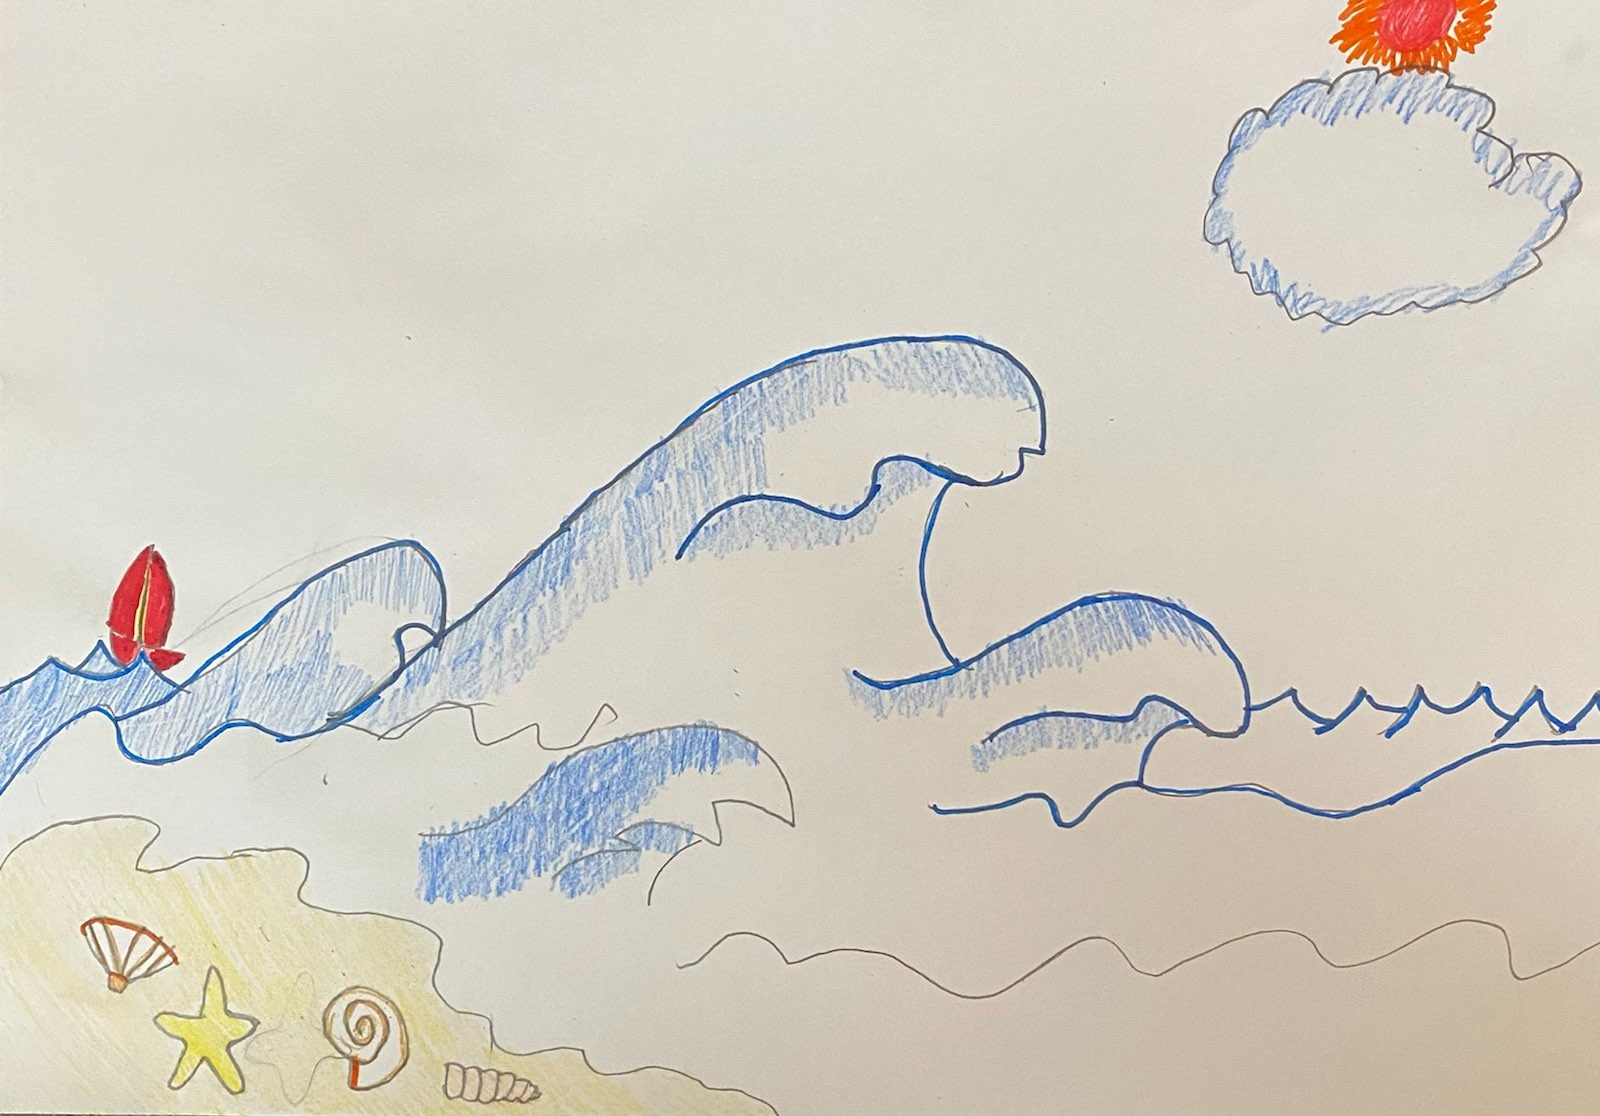
\includegraphics[width=\paperwidth]{assets/cover.jpg}}
    };
\end{tikzpicture}

%%%%%%%%%%%%%%%%%%%%%%%%%%%%%%%%%%%%%%%%%%%%%%%%%%%%%%%%%%%%%%%%%%%%%%%%%%%%%%%
% Table of Contents
%%%%%%%%%%%%%%%%%%%%%%%%%%%%%%%%%%%%%%%%%%%%%%%%%%%%%%%%%%%%%%%%%%%%%%%%%%%%%%%

\clearpage
\tableofcontents
\clearpage

%%%%%%%%%%%%%%%%%%%%%%%%%%%%%%%%%%%%%%%%%%%%%%%%%%%%%%%%%%%%%%%%%%%%%%%%%%%%%%%
% Sections
%%%%%%%%%%%%%%%%%%%%%%%%%%%%%%%%%%%%%%%%%%%%%%%%%%%%%%%%%%%%%%%%%%%%%%%%%%%%%%%

%%%%%%%%%%%%%%%%%%%%%%%%%%%%%%%%%%%%%%%%%%%%%%%%%%%%%%%%%%%%%%%%%%%%%%%%%%%%%%%%%%%%%%%%%%%%%%%%%%%%
% Data Types
%%%%%%%%%%%%%%%%%%%%%%%%%%%%%%%%%%%%%%%%%%%%%%%%%%%%%%%%%%%%%%%%%%%%%%%%%%%%%%%%%%%%%%%%%%%%%%%%%%%%

\section{Data Types}

We have different kinds of built-in \textit{things} in Python. These \textit{things} are called data
types.
\newline
Here is their table:

\begin{table}[H]
    \begin{tabular}{p{0.15\linewidth}p{0.25\linewidth}p{0.60\linewidth}}
        \toprule
        \textbf{Data Type} & \textbf{Category} & \textbf{Examples}\\
        \midrule

        \mintinline{python}{bool} & Boolean & \mintinline{python}{False}, \mintinline{python}{True}\\
        \midrule

        \mintinline{python}{int} & Integers & 1, 2, 3, -1, -2, -3, 0\\
        \midrule

        \mintinline{python}{float} & Floating point numbers & 0.5, 1.5, 2.5, -0.5, -1.5, -2.5\\
        \midrule

        \mintinline{python}{complex} & Complex numbers & \(1 + i\), \(2 + 2i\), \(-3 + 5i\)\\
        \midrule

        \mintinline{python}{str} & Text sequence type & \mintinline{python}{"a"},
                                                        \mintinline{python}{"abc"},
                                                        \mintinline{python}{"Hello, world!"}\\
        \midrule

        \mintinline{python}{list} & Sequence type & \mintinline{python}{[]},
                                                    \mintinline{python}{[0]},
                                                    \mintinline{python}{[1, 2, 3]},
                                                    \mintinline{python}{["ab", "bc", "cd"]}\\
        \midrule

        \mintinline{python}{tuple} & Sequence type & \mintinline{python}{()},
                                                     \mintinline{python}{(0)},
                                                     \mintinline{python}{(1, 2, 3)},
                                                     \mintinline{python}{("ab", "bc", "cd")}\\
        \midrule

        \mintinline{python}{range} & Sequence type & \mintinline{python}{range(10)},
                                                     \mintinline{python}{range(1, 10)},
                                                     \mintinline{python}{range(3, 8, 2)}}\\
        \midrule

        \mintinline{python}{set} & Set type & \mintinline{python}{{}},
                                              \mintinline{python}{{0}},
                                              \mintinline{python}{{1, 2, 3}},
                                              \mintinline{python}{{"ab", "bc", "cd"}}\\
        \midrule

        \mintinline{python}{frozenset} & Set type & \mintinline{python}{frozenset({})},
                                                    \mintinline{python}{frozenset({0})},
                                                    \mintinline{python}{frozenset({1, 2, 3})}\\
        \midrule

        \mintinline{python}{dict} & Mapping type & \mintinline{python}{{}},
                                                   \mintinline{python}{{0: 1}},
                                                   \mintinline{python}{{2: 3, 4: 5}},
                                                   \mintinline{python}{{"a": 0, "b": 1, "c": 2}}\\
        \bottomrule
    \end{tabular}
    \caption{Built-in Data Types}
    \label{tb.data.types}
\end{table}

\subsection{\mintinline{python}{bool}}

This is great.

%%%%%%%%%%%%%%%%%%%%%%%%%%%%%%%%%%%%%%%%%%%%%%%%%%%%%%%%%%%%%%%%%%%%%%%%%%%%%%%%%%%%%%%%%%%%%%%%%%%%
% The `print` Function
%%%%%%%%%%%%%%%%%%%%%%%%%%%%%%%%%%%%%%%%%%%%%%%%%%%%%%%%%%%%%%%%%%%%%%%%%%%%%%%%%%%%%%%%%%%%%%%%%%%%

\section{The \mintinline{python}{print} Function}

Just like in math, we have functions in Python as well. While we will cover Python functions in a
greater detail in later chapters, the \mintinline{python}{print} function is so useful that we will
start by learning how it works!

\begin{minted}{python}
    >>> print("Hello, world!")
    Hello, world!
\end{minted}

The way \mintinline{python}{print} works is that you write out these characters
\mintinline{python}{p-r-i-n-t}, followed by the left paren \mintinline{python}{(}, followed by
whatever we want to print, and finally the right paren \mintinline{python}{)}.

\begin{minted}{python}
    >>> print(0)
    0
    >>> print(1)
    1
    >>> print(9)
    9
    >>> print(10)
    10
\end{minted}


%%%%%%%%%%%%%%%%%%%%%%%%%%%%%%%%%%%%%%%%%%%%%%%%%%%%%%%%%%%%%%%%%%%%%%%%%%%%%%%
% The End of the Document
%%%%%%%%%%%%%%%%%%%%%%%%%%%%%%%%%%%%%%%%%%%%%%%%%%%%%%%%%%%%%%%%%%%%%%%%%%%%%%%

\end{document}
